\documentclass[a4paper,10pt]{article}

\usepackage{url}
\usepackage{parskip} 	

%other packages for formatting
\RequirePackage{color}
\RequirePackage{graphicx}
\usepackage[usenames,dvipsnames]{xcolor}
\usepackage[scale=0.9]{geometry}

%tabularx environment
\usepackage{tabularx}

%for lists within experience section
\usepackage{enumitem}

% centered version of 'X' col. type
\newcolumntype{C}{>{\centering\arraybackslash}X} 

%to prevent spillover of tabular into next pages
\usepackage{supertabular}
\usepackage{tabularx}
\newlength{\fullcollw}
\setlength{\fullcollw}{0.47\textwidth}

%custom \section
\usepackage{titlesec}				
\usepackage{multicol}
\usepackage{multirow}

%CV Sections inspired by: 
%http://stefano.italians.nl/archives/26
\titleformat{\section}{\Large\scshape\raggedright}{}{0em}{}[\titlerule]
\titlespacing{\section}{0pt}{0pt}{10pt}

%for publications
\usepackage[style=authoryear,sorting=ynt, maxbibnames=2]{biblatex}

%Setup hyperref package, and colours for links
\usepackage[unicode, draft=false]{hyperref}
\definecolor{linkcolour}{rgb}{0,0.2,0.6}
\hypersetup{colorlinks,breaklinks,urlcolor=linkcolour,linkcolor=linkcolour}
\addbibresource{citations.bib}
\setlength\bibitemsep{1em}

\usepackage{float}

%for social icons
\usepackage{fontawesome5}

\pagestyle{empty} 

%----------------------------------------------------------------------------------------
%	TITLE
%----------------------------------------------------------------------------------------

% \begin{tabularx}{\linewidth}{ @{}X X@{} }
% \huge{Your Name}\vspace{2pt} & \hfill \emoji{incoming-envelope} email@email.com \\
% \raisebox{-0.05\height}\faGithub\ username \ | \
% \raisebox{-0.00\height}\faLinkedin\ username \ | \ \raisebox{-0.05\height}\faGlobe \ mysite.com  & \hfill \emoji{calling} number
% \end{tabularx}

\newcommand{\name}{Khushvind Maurya} % Your Name
\newcommand{\course}{Bachelor of Technology} % Your Course
\newcommand{\roll}{2021MT10238} % Your Roll No.
\newcommand{\phone}{7652041595} % Your Phone Number
\newcommand{\emaila}{khushvind.pro@gmail.com} %Email 1
\newcommand{\emailb}{mt1210238@iitd.ac.in} %Email 2
\newcommand{\github}{khushvind} %Github
% \newcommand{\website}{} %Website
\newcommand{\linkedin}{khushvind-maurya} %linkedin




\begin{document}
\fontfamily{cmr}\selectfont
%----------HEADING-----------------
\parbox{2.35cm}{
    \centering
    
\includegraphics[width=2cm]{iitd logo.png}
}
\hfill
\parbox{\dimexpr\linewidth-5.2cm\relax}{
    \parbox{0.6\linewidth}{
        \textbf{\LARGE \name}\\[4pt]
        \course\\
        Mathematics and Computing
    }
    \hfill
    \parbox{0.35\linewidth}{
        \raggedleft
        +91-\phone\\
        \href{mailto:\emaila}{\emaila}\\
        \href{https://linkedin.com/in/khushvind-maurya}
        {\faLinkedin\ khushvind-maurya}\\
        \href{https://github.com/khushvind}
        {\faGithub\ khushvind}
    }
}
\hfill
\parbox{2.35cm}{
    \centering
    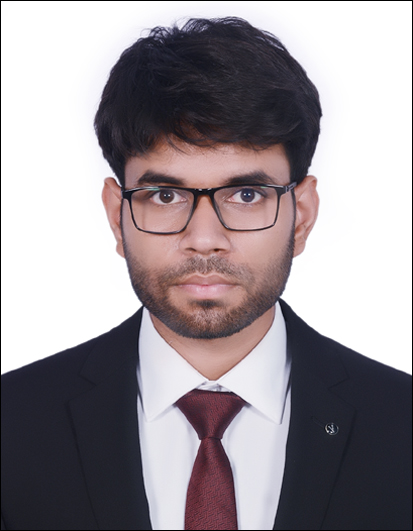
\includegraphics[width=1.8cm]{pic.JPG}
}



% \begin{tabularx}{\linewidth}{@{} C @{}}
% \Huge{KHUSHVIND MAURYA} \\[7.5pt]
% % \href{https://github.com/khushvind}{\raisebox{-0.05\height}\faGithub\ khushvind} \ $|$ \ 
% \href{https://linkedin.com/in/khushvind-maurya}{\raisebox{-0.05\height}\faLinkedin\ khushvind-maurya} \ $|$  \ 
% \href{mailto:khushvind.iitd@gmail.com}{\raisebox{-0.05\height}\faEnvelope \ khushvind.iitd@gmail.com} \ $|$ \ 
% \href{tel:+917652041595}{\raisebox{-0.05\height}\faMobile \ +917652041595} \\
% \end{tabularx}

%----------------------------------------------------------------------------------------
% EXPERIENCE SECTIONS
%----------------------------------------------------------------------------------------

\section{\textbf{Academic Details}}
% \begin{table}[H]
\setlength{\tabcolsep}{13pt}

\begin{tabularx}{\linewidth}{l  X  X  r}
\centering
% \textbf{Year} & \textbf{Degree/Board} & \textbf{Institute} & Grade\\
% 2021 - (Expected 2025) & B.Tech Mathematics and Computing at \textbf{IIT Delhi} \hfill \normalsize (GPA: 8.08/10.0 (current)) \\
\textbf{Year} & \textbf{Degree/Course} & \textbf{Institute} & \textbf{GPA/Marks(\%)} \\
2021-25  & B.Tech Mathematics and Computing & Indian Institute Of Technology Delhi & 8.07/10.0 \\
2021 & CBSE (Class XII) & Disha Delphi Public School & 95.6\% \\
2019 & CBSE (Class X) & Dewan Public School & 95.6\%
\end{tabularx}

\section{\textbf{Experience}}
\textbf{Salesforce $\mid$ Revenue Cloud:} \textit{Software Engineer $\mid$ Associate Member Of Technical Staff}\hfill\textit{(June 2025-Present) }\\
- Worked on \textbf{Revenue Cycle Management} with a focus on building and enhancing the billing and pricing infrastructure\\
- Built \textbf{Billing Collection Agent} on \textbf{Agentforce}, and designed invocable actions to automate billing account summaries\\
- Contributed to \textbf{Salesforce Go}, reducing cloud setup time by \textbf{98\%} via automated configuration and record provisioning\\
- Owned \textbf{Revenue Cloud Growth license} support in \textbf{Salesforce Go}, integrating with automation and provisioning flows
% - Collaborated with \textbf{cross-functional teams}, debugging, \textbf{resolving critical production issues}, and improving reliability
% - Collaborated with \textbf{cross-functional teams} (Product, QA, and DevOps) to deliver high-quality, customer-centric features\\
% - \textbf{Enhanced overall test coverage} by implementing unit, integration, and end-to-end tests to maintain system robustness
% - Enhanced test coverage with unit, integration, and end-to-end tests to maintain system robustness
% - Enhanced overall test coverage by implementing comprehensive unit, integration, and end-to-end tests, improving system robustness, reducing regression issues, and ensuring reliable functionality across critical billing and pricing workflows.
% - Developed and optimized backend services for large-scale subscription billing and invoicing, ensuring accuracy and compliance with financial standards.\\
% - Improved performance of pricing engine by refactoring core components, reducing computation time and enhancing scalability for enterprise clients. \\ 
% - Designed and implemented APIs to integrate Revenue Cloud with external financial and CRM systems.\\
% - Participated in code reviews and design discussions to maintain coding standards and system scalability.\\
\section{\textbf{Internships}}
\textbf{Samsung Research Institute - Bangalore $\mid$ OnDevice AI Team:} \textit{Software Developer Intern}\hfill\textit{(May 2024-July 2024) }\\
- Collaborated with Samsung’s OnDevice AI Team to \textbf{enhance quantization tools} for optimizing AI models on devices\\
- Developed features to extract the encoding values and files from different \textbf{ONNX} and \textbf{TFLite} LLMs post-quantization\\
- Implemented \textbf{AIMET}-like encoding file generation, ensuring compatibility and smooth integration with existing workflows\\
- Conducted extensive testing to maintain final model accuracy \textbf{within $\textbf{2\%}$} deviation from the original floating-point model\\
% - Conducted extensive testing and validation of quantized models to ensure accuracy and efficiency in real-world applications\\
\textbf{Australian National University $\mid$ Prof. Ahad N. Zehmakan:} \textit{Research Intern}\hfill\textit{(May 2023-July 2023) } \\
- Worked on \textbf{source-agnostic algorithms} to minimize the dissemination of misinformation across \textbf{large social networks}\\
% - \textbf{Data mining} and \textbf{Knowledge Discovery} to gather valuable information about the social network datasets used. \\
- Implemented the \textbf{Independent Cascade Diffusion Model} to simulate the spread of misinformation in social networks\\
% - Used different community detection algorithms, like \textbf{Louvain} and \textbf{Leiden} to detect communities in social networks\\
- Proposed an algorithm that consistently improved the containment factor by \textbf{at least $\textbf{60\%}$} compared to existing algorithms\\
% - The outcome of the project was published in the paper titled \textbf{`Mitigating Misinformation Spreading in Social Networks Via Edge Blocking'} at the Pacific Rim International Conference on Artificial Intelligence (\textbf{PRICAI}) 2023.
- The results were published at the prestigious \textbf{Pacific Rim International Conference on Artificial Intelligence}, 2023
\section{\textbf{Key Projects}}
\textbf{OpenHands $\mid$ Open Source Project $\mid$ Prof. G. Neubig (Carnegie Mellon University)}\hfill\textit{(June 2024 - Aug 2024)} \href{https://github.com/khushvind/OpenDevin}{\raisebox{-0.05\height}\faGithub}\\
- Integrated \textbf{MemGPT}-like functionality into OpenHands's \textbf{Short Term} Memory to address context window exceed errors\\
- Implemented a \textbf{Condenser} to dynamically condense event stream as the token size approaches the context window limit\\
- Developed it to work seamlessly with the \textbf{agent controller}, ensuring efficient integration with existing, and future agents\\
- Experimented with various methods to effectively identify events for condensation, optimizing the performance of the agent\\
\textbf{Quantization of Large Language Models $\mid$ Custom W8A16 Quantizer for LLM Optimization} \hfill\textit{(May 2024)} \href{https://github.com/khushvind/Quantization-LLMs}{\raisebox{-0.05\height}\faGithub}\\
- Made a custom \textbf{W8A16 quantizer} specifically designed to quantize NN weights to 8-bit and activations to 16-bit precision\\
- Implemented it within the PyTorch framework, ensuring seamless integration and compatibility with existing architectures\\
% - It replaces the $torch.nn.Linear$ layers with a $W8A16LinearLayer$, optimizing both storage and computational efficiency\\
- Achieved a \textbf{memory footprint reduction} of over $\textbf{40\%}$ in models, boosting both storage and computational efficiency\\
\textbf{Virtual Memory Simulator - TLB Allocator $\mid$ Prof. Ashutosh Rai}\hfill\textit{(Sept 2024 - Oct 2024)} \href{https://github.com/khushvind/Virtual_Memory_Simulator-TLB_Allocator}{\raisebox{-0.05\height}\faGithub}\\
- Developed a simulator that models the behavior of four \textbf{TLB} replacement algorithms, \textbf{FIFO}, \textbf{LIFO}, \textbf{LRU}, and \textbf{Optimal}\\
- Utilized \textbf{low-level system} calls to manage heap memory, handling memory requests dynamically with custom algorithms\\
- Implemented a \textbf{custom memory allocator} that replicates the functionality of standard \textbf{malloc}, \textbf{calloc}, and \textbf{free} in C\\
% \textbf{Dynamic CPU Process Scheduling Algorithms in C $\mid$ Prof. Ashutosh Rai}\hfill\textit{(Aug 2024 - Sept 2024)} \href{https://github.com/khushvind/CPU-Process-Scheduler}{\raisebox{-0.05\height}\faGithub}\\
% - Developed a CPU Process Scheduler, implementing key scheduling algorithms including \textbf{FCFS}, \textbf{RR}, \textbf{MLFQ}, and \textbf{SJF}\\
% - Implemented \textbf{real-time} input handling, demonstrating proficiency in event-driven programming and I/O management\\
% - Generated detailed performance metrics (burst time, turnaround time, waiting time, and response time) for each scheduler\\
% \textbf{OS Utility: Interactive Shell with Enhanced Features $\mid$ Prof. Ashutosh Rai}\hfill\textit{(July 2024 - Aug 2024)} \href{https://github.com/khushvind/Custom-Linux-Shell}{\raisebox{-0.05\height}\faGithub}\\
% - Implemented a UNIX-like shell using C, that interactively accepts the inputs and supports commands like ls, cd, mkdir\\
% - Added functionalities to run \textbf{background commands}, support \textbf{piping between commands} and support \textbf{env variables}\\
% - Integrated critical built-in features, including directory navigation, command history, and robust error-handling mechanisms\\
\textbf{Predictive Modeling for Student Grades $\mid$ Prof. Bhawani Sankar Panda} \hfill\textit{(Mar 2024 - Apr 2024)} \href{https://github.com/khushvind/MTL782-Data-Mining/tree/main/A1}{\raisebox{-0.05\height}\faGithub}\\
- Developed a model to predict the final grade of students in a course based on their initial performance, and attendance\\
- Utilized TensorFlow Decision Forests (\textbf{TF-DF}) library to train \textbf{Random Forest} and \textbf{Gradient Boosted Trees} models\\
- Performed\textbf{ hyperparameter tuning} on the models to achieve an impressive accuracy of more than $\textbf{85\%}$ on both models\\
% \textbf{Oceanic Data Analysis: Cyclone Features and Temperature Progression $\mid$ Prof. Samiran Mandal} \textit{(March 2023)}\\
% - Analyzed \textbf{GHRSST} and \textbf{HYCOM} datasets from APDRC to study trends in weather at different locations on the ocean\\
% - Identified the location of `Severe Cyclonic Storm' for a given cyclone, halocline and thermocline, using the datasets\\
% - Conducted linear regression, revealing a temperature increase of 0.0365°C/year, indicating the effects of global warming
\textbf{Adversarial Search $\mid$ Chess Bot Using Minimax Algorithm with Alpha-Beta Pruning} \hfill\textit{(Dec 2024 - Jan 2025)} \href{https://github.com/khushvind/Adversarial-Search--Chess-Bot-Using-Minimax-Algorithm-with-Alpha-Beta-Pruning}{\raisebox{-0.05\height}\faGithub}\\
- Designed a chess bot leveraging the Minimax algorithm with Alpha-Beta pruning for efficient and optimal move evaluation\\
% - Developed core functionalities including bot-vs-bot and bot-vs-user interactions, with real-time chessboard visualization using Python libraries (chess, IPython.display, and ipywidgets).
- Optimized game tree evaluation using Alpha-Beta pruning, reducing computational overhead while maintaining accuracy\\
\textbf{Search Nearby Program $\mid$ Prof. Ashish Chiplunkar \& Prof. Naveen Garg}\hfill\textit{(Sept 2022 - Oct 2022)} \href{https://github.com/khushvind/COL106-Assignments/tree/main/Assignment%203}{\raisebox{-0.05\height}\faGithub}\\
- Implemented a `\textbf{Point Database}' to store the position of all the landmarks in the map using \textbf{Range Tree} Data Structure\\
- The program efficiently stored landmark data for fast processing of \textit{``search nearby"} queries, similar to Google Maps\\
- Handled range queries in $O(m + log^2(n))$ time, where n is the number of data points and m is the total points returned

\section{\textbf{Skills}}
\textbf{Programming Languages:} Python, C/C++, Java, MATLAB $\mid$ \textbf{Libraries:} Numpy, Pandas, TensorFlow, Scikit-Learn, PyTorch, Matplotlib, NLTK, AIMET, Networkx, Networkit $\mid$ \textbf{Softwares:} Git, Bash, Linux, Docker, AWS Bedrock, LaTeX

\section{\textbf{Scholastic Achievements}}
- \textbf{Nikunj Agarwal Memorial Scholarship 2023-24:} Awarded the scholarship by IIT Delhi, for academic year 2023-24.\\
- \textbf{JEE Advanced 2021:} Secured an \textbf{All India Rank of 302} among the selected pool of students in JEE Main 2021.\\
- \textbf{JEE Main 2021:} Qualified with an \textbf{All India Rank of 493} (99.96 percentile) among 1 million candidates all over India.\\
- \textbf{KVPY Fellowship 2020:} Conferred by IISc, and DST, Government of India, rewarded for scientific acumen and aptitude.\\
- \textbf{INESO 2019 (Anna University $\&$ GSI):} Secured an All India Rank of 22 and qualified for the next stage, OCSC.\\
- \textbf{INAO Jr 2018 (HBCSE):} Secured a rank among the top 21 students all over India and qualified for next stage, OCSC.

\section{\textbf{Courses}}
\textbf{Completed:} Introduction To Computer Science, Probability \& Stochastic Processes, Data Structures \& Algorithms, Analysis \& Design of Algorithms, Computer Architecture, Cloud Computing, Linear Algebra \& Differential Equations, Optimization Methods \& Applications, Data Mining, Statistical Methods, Cryptography, Real And Complex Analysis, Fuzzy Sets And Applications, Numerical And Computational Methods in Research, Digital Electronics, Discrete Mathematical Structures, Principles Of Electronic Materials, Financial Mathematics,  Macro Economics, Operating Systems, Theory Of Computation, Game Theory, Numerical Methods $\&$ Computation, Functional Analysis, Computational Methods For Differential Equations
\section{\textbf{Organizations/Extracurriculars}}
\textbf{Mathematics Society, IIT Delhi:} \textit{Coordinator} \textit{(June 2023 - May 2024)} - Responsible for coordinating various society events $|$ \textit{Executive} \textit{(June 2022 - May 2023)} - Planned and organized many society events year-round \\
\textbf{TRYST, IIT Delhi:} \textit{Coordinator} \textit{(Nov 2023 - May 2024)} - Coordinator in the Admin and Finance Vertical in TRYST 2024, North India's largest technical fest, hosted by IIT Delhi. Responsible for revamping the finance and budget model to boost revenue and coordinating logistics of 20+ hybrid events. \\
\textbf{Hostel Technical Committee:} \textit{Member (June 2023 - May 2024)} - Responsible for managing and maintaining the hostel website, and other tech-related requirements.\\
\textbf{Rendezvous, IIT Delhi:} \textit{Activity Head (2023)} Managed the hospitality team and successfully conducted 10+ events during Rendezvous\\

% \textbf{Hostel Cultural Committee Member:} \textit{(June 2022 - May 2023)} - Responsible for promoting extracurricular activities among the hostel residents and planning and executing events year-round.\\


\vfill


\end{document}


